% demo
\begin{frame}[plain,noframenumbering]
    \centering
    \vspace{0.35cm}

    {\Large\color{mainblue}\textbf{Package Demonstration}}

    \vspace{0.15cm}
    {\scriptsize KFCProcedure Workflow and Usage Example}

    \vspace{0.35cm}

    \href{run:videos/demo.mp4}{
        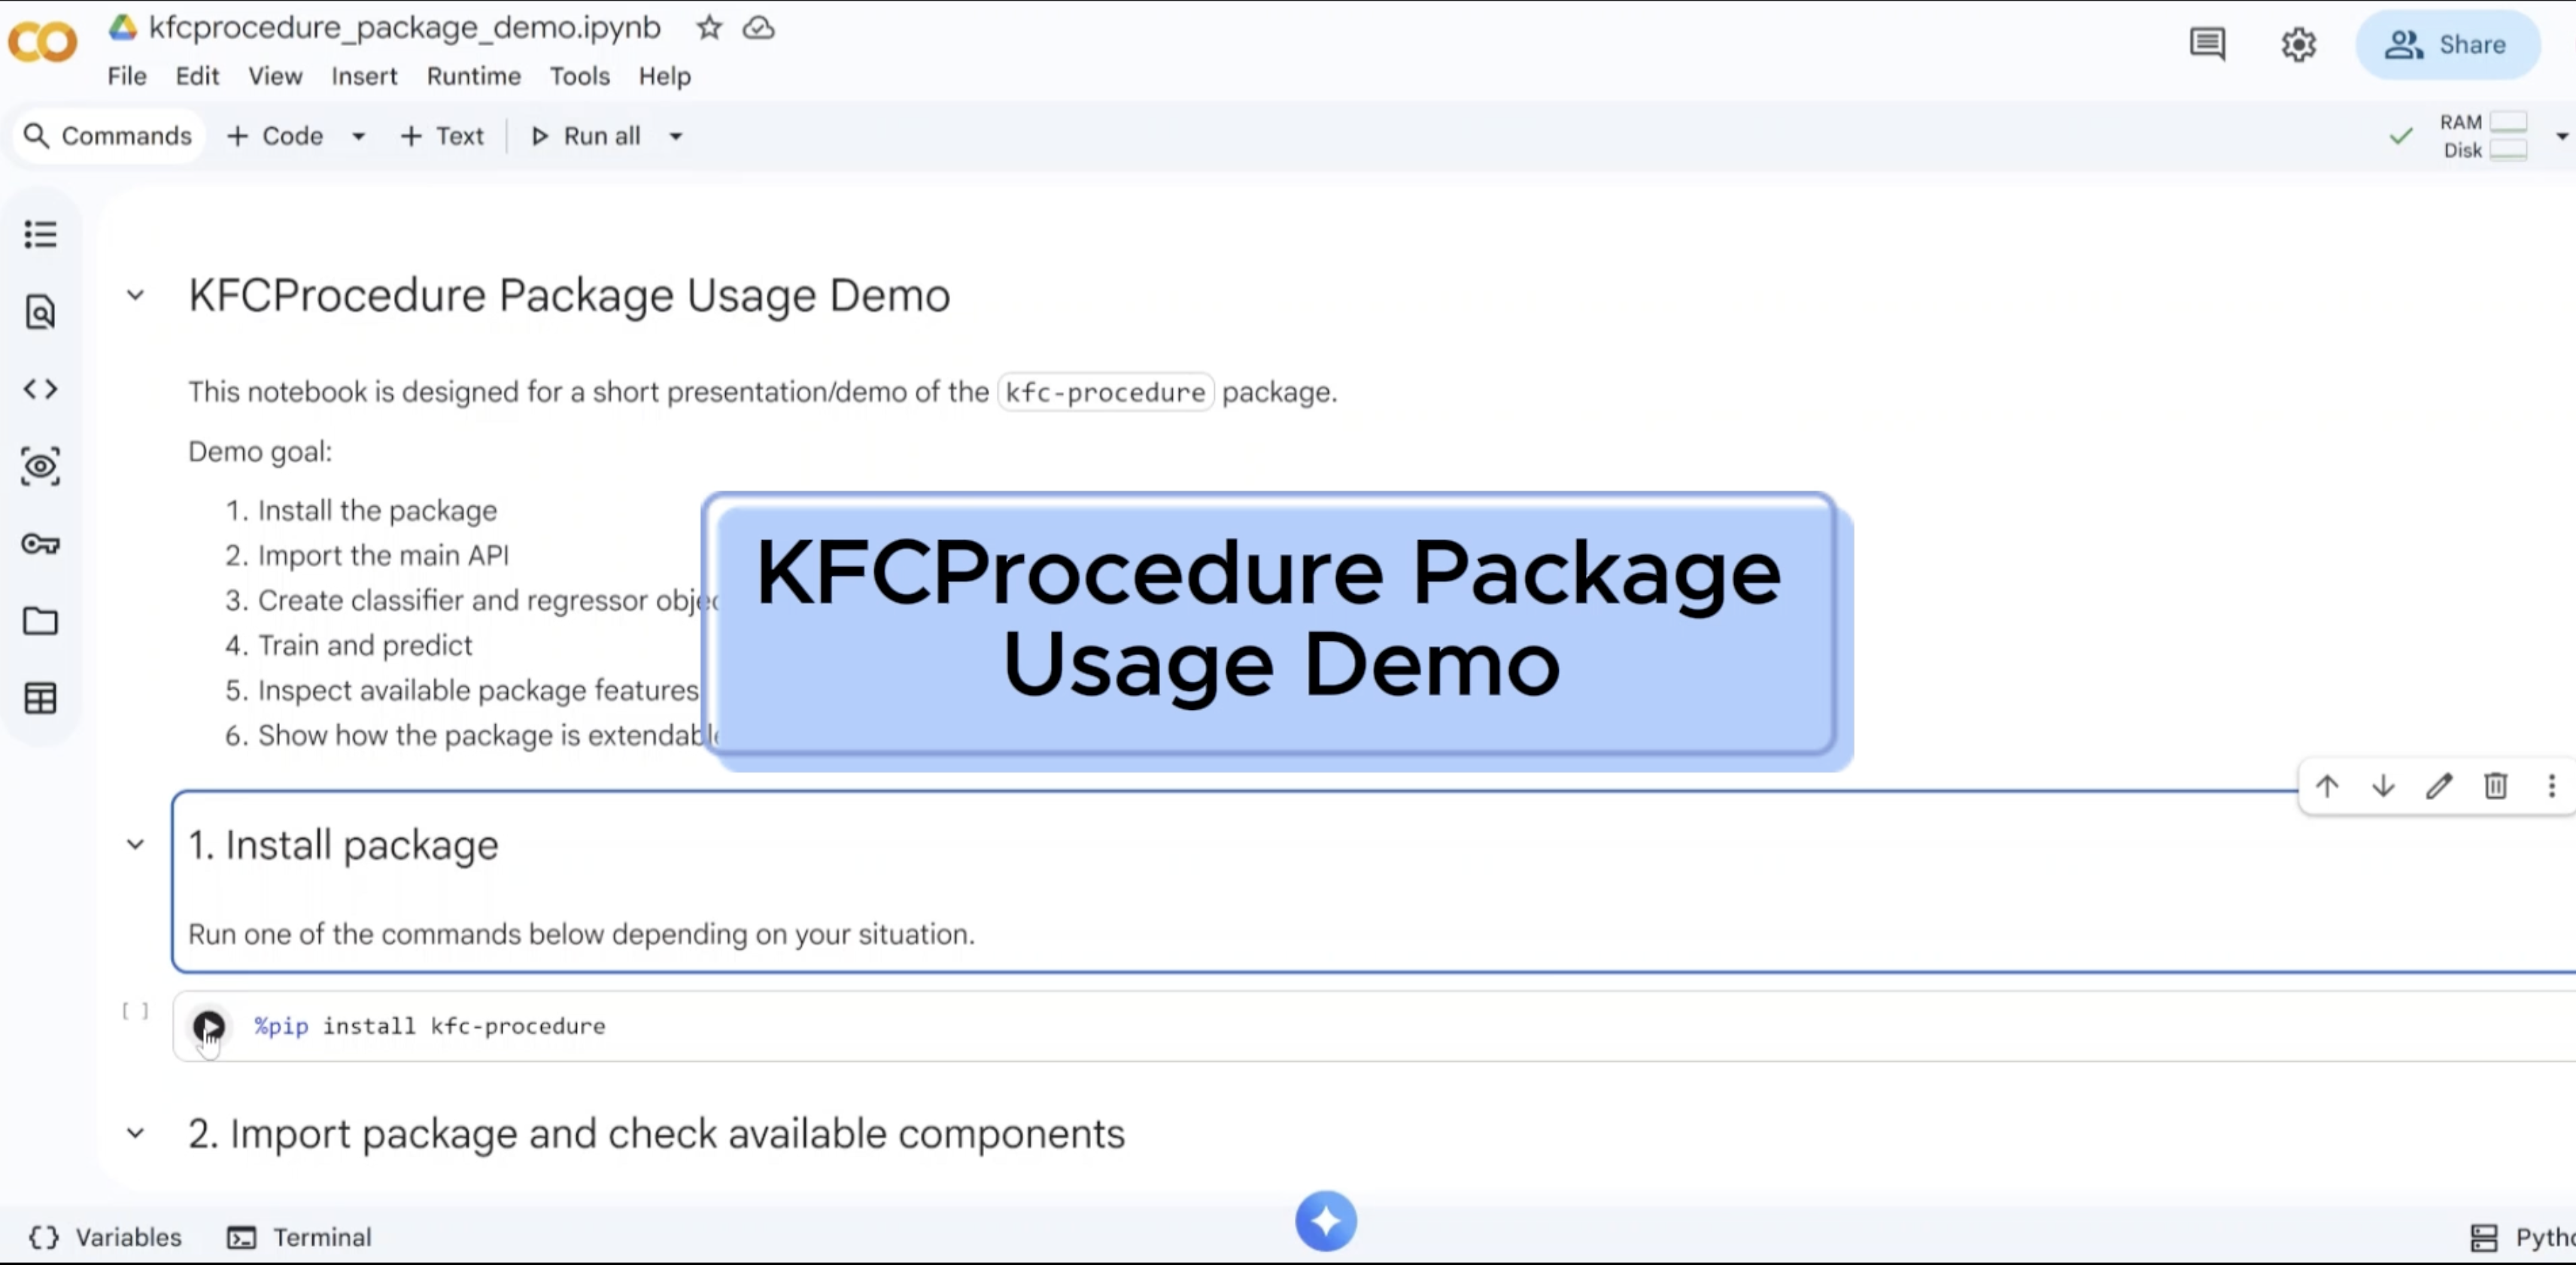
\includegraphics[width=0.68\textwidth]{figures/demo_thumbnail.png}
    }
\end{frame}

% references slide
\begin{frame}[plain,noframenumbering]

    \vspace{-0.5cm}
    \large\color{mainblue}\textbf{References}
    \vspace{0.2cm}
    \printbibliography[heading=none]

\end{frame}

% thank you slide
\begin{frame}[plain,noframenumbering]

    \begin{tikzpicture}[remember picture,overlay]
        \node[opacity=0.06] at (current page.center)
        {
\includegraphics[width=0.45\paperwidth]{figures/schools/watermark.png}};
    \end{tikzpicture}

    % QR code at bottom
    \begin{tikzpicture}[remember picture,overlay]
        \node[anchor=south east] at ([xshift=-0.65cm,yshift=0.45cm]current page.south east) {
            \begin{minipage}{3.2cm}
                \centering
                
\includegraphics[width=1.85cm]{figures/qr_google_doc_resources.png}

                \vspace{0.08cm}

                {\tiny Scan for resources}
            \end{minipage}
        };
    \end{tikzpicture}

    \centering
    \vfill

    {\Huge\bfseries\color{mainblue}Thank You!}

    \vspace{0.45cm}

    {\Large Questions and Answers}

    \vspace{0.65cm}

    {\small Python Libraries for Clusterwise Predictive Models: KFCProcedure and GradientCOBRA}

    \vfill
\end{frame}

% appendix slide
\begin{frame}[plain,noframenumbering]

    \centering
    \vspace{2.2cm}
    \Huge\color{mainblue}\textbf{Appendix}

    \vspace{0.35cm}

    {\large Additional Technical Details}

\end{frame}

\begin{frame}[plain,noframenumbering]
    \scriptsize

    \vspace{-0.35cm}

    {\Large\color{mainblue}\textbf{Appendix A: KFCProcedure Formulation}}

    \vspace{0.25cm}

    \begin{columns}[T,onlytextwidth]

        % =========================
        % Column 1: K-step
        % =========================
        \column{0.31\textwidth}

        \begin{block}{1. K-step: Cluster}
            For a convex function \(\phi\), the Bregman divergence is:
            \[
                D_{\phi}(x,\mu)
                =
                \phi(x)-\phi(\mu)
                -
                \langle \nabla \phi(\mu), x-\mu \rangle
            \]

            Each observation is assigned to the nearest cluster:
            \[
                \mathcal{C}_{m,k}
                =
                \left\{
                i :
                k =
                \arg\min_{\ell}
                D_m(x_i,\mu_{m,\ell})
                \right\}
            \]

            {\tiny
                This step discovers local structures using divergence-based clustering, such as Euclidean, generalized KL, Itakura--Saito, or logistic divergence.
            }
        \end{block}

        % =========================
        % Column 2: F-step
        % =========================
        \column{0.31\textwidth}

        \begin{block}{2. F-step: Local Model}
            A supervised model is trained inside each discovered cluster:
            \[
                f_{m,k}
                =
                \arg\min_{f \in \mathcal{F}}
                \sum_{i \in \mathcal{C}_{m,k}}
                \ell(y_i,f(x_i))
            \]

            {\tiny
                This step learns specialized supervised models for each local group.
            }
        \end{block}

        % =========================
        % Column 3: C-step
        % =========================
        \column{0.31\textwidth}

        \begin{block}{3. C-step: Combination}
            For a new sample \(x\), select the nearest local model:
            \[
                k_m^*(x)
                =
                \arg\min_k
                D_m(x,\mu_{m,k})
            \]

            \[
                z_m(x)
                =
                f_{m,k_m^*(x)}(x)
            \]

            Final prediction:
            \[
                \hat{y}(x)
                =
                C(z_1(x),\ldots,z_M(x))
            \]

            {\tiny
                This step combines local predictions using a combiner.
            }
        \end{block}

    \end{columns}

    \vspace{0.25cm}

    {\tiny
        \textbf{Interpretation:}
        KFCProcedure discovers local structures, trains local supervised models, and combines their predictions through the C-step.
        \cite{has2021kfc}
    }

\end{frame}

\begin{frame}[plain,noframenumbering]
    \scriptsize
    \vspace{-0.25cm}
    {\Large\color{mainblue}\textbf{Appendix B: GradientCOBRA Implementation Formulation}}

    \vspace{0.25cm}

    \renewcommand{\arraystretch}{1.18}
    \setlength{\tabcolsep}{2.2pt}

    \begin{tabularx}{\textwidth}{
            >{\raggedright\arraybackslash}p{3.25cm}
            >{\raggedright\arraybackslash}X
            >{\raggedright\arraybackslash}p{4.75cm}}
        \toprule
        \textbf{Step} & \textbf{Implementation Meaning}                                                & \textbf{Formula} \\
        \midrule

        1. Input Data
                      & Input features and target values.
                      &
        \( \mathcal{D}=\{(x_i,y_i)\}_{i=1}^{n} \)                                                                         \\

        2. Splitter
                      & Split data into estimator-training data and aggregation data.
                      &
        \( \mathcal{D}=\mathcal{D}_k \cup \mathcal{D}_l \)                                                                \\

        3. Estimators
                      & Train base estimators on \(\mathcal{D}_k\), then predict on \(\mathcal{D}_l\).
                      &
        \( r(x)=\big(r_1(x),\ldots,r_M(x)\big) \)                                                                         \\

        4. Normalize Constant
                      & Scale prediction-space values before distance computation.
                      &
        \( c=\dfrac{30}{(\max_i |y_i|+\epsilon)M} \),
        \quad
        \( \tilde{r}(x)=c\,r(x) \)                                                                                        \\

        5. Distance Module
                      & Compute distances in normalized prediction space.
                      &
        \( D_{qi}=d\big(\tilde{r}(x_q),\tilde{r}(x_i)\big) \)                                                             \\

        6. Kernel Adapter
                      & Apply one-parameter bandwidth scaling.
                      &
        \( D'_{qi}=bD_{qi} \)                                                                                             \\

        7. Kernel
                      & Convert distance into similarity weights.
                      &
        \( W_{qi}=K(D'_{qi}) \),
        \quad default:
        \( K(D')=\exp(-D') \)                                                                                             \\

        8. Optimize and Loss
                      & Select the best bandwidth using cross-validation loss.
                      &
        \( b^*=\arg\min_b
        \frac{1}{V}
        \sum_{q\in \mathcal{V}}
        \mathcal{L}\big(y_q,\hat{y}_b(x_q)\big) \)                                                                        \\

        9. Aggregation
                      & Aggregate target values using kernel weights.
                      &
        \( \hat{y}(x_q)=
        \dfrac{
            \sum_{i\in\mathcal{D}_l} W_{qi}y_i
        }{
            \sum_{i\in\mathcal{D}_l} W_{qi}
        } \)                                                                             \\

        10. Output
                      & Return final prediction.
                      &
        \( \hat{y}(x_q) \)                                                                                                \\

        \bottomrule
    \end{tabularx}

    \vspace{0.12cm}

    {\tiny
        \textbf{Implementation note:}
        In this package, GradientCOBRA trains base estimators, maps samples into prediction space,
        normalizes predictions, computes a distance matrix, scales it using a bandwidth adapter,
        applies a kernel, optimizes bandwidth by validation loss, and returns a weighted aggregation.
        \cite{biau2016,has2023gradientcobra}
    }

\end{frame}

\begin{frame}[plain,noframenumbering]
    \scriptsize
    \vspace{-0.25cm}

    {\Large\color{mainblue}\textbf{Appendix C: Distance and Kernel Modules}}

    \begin{columns}[T,onlytextwidth]

        \column{0.48\textwidth}
        \begin{block}{Distance Module}
            \renewcommand{\arraystretch}{1.18}
            \setlength{\tabcolsep}{2pt}
            \begin{tabularx}{\linewidth}{p{2.0cm} X}
                \toprule
                \textbf{Distance} & \textbf{Formula}                    \\
                \midrule

                Euclidean
                                  &
                \( d(x,y)=\sqrt{\sum_j (x_j-y_j)^2} \)                  \\

                Manhattan
                                  &
                \( d(x,y)=\sum_j |x_j-y_j| \)                           \\

                Minkowski
                                  &
                \( d_p(x,y)=\left(\sum_j |x_j-y_j|^p\right)^{1/p} \)    \\

                Cosine
                                  &
                \( d(x,y)=1-\dfrac{x^\top y}{\|x\|\|y\|+\varepsilon} \) \\

                Hamming
                                  &
                \( d(x,y)=\dfrac{1}{d}\sum_j \mathbf{1}(x_j\neq y_j) \) \\

                \bottomrule
            \end{tabularx}
        \end{block}

        \column{0.48\textwidth}
        \begin{block}{Kernel Module}
            \renewcommand{\arraystretch}{1.18}
            \setlength{\tabcolsep}{2pt}
            \begin{tabularx}{\linewidth}{p{2.0cm} X}
                \toprule
                \textbf{Kernel} & \textbf{Formula}   \\
                \midrule

                Radial / RBF
                                &
                \( K(D)=\exp(-D^2) \)                  \\

                Exponential
                                &
                \( K(D)=\exp(-D^\alpha) \)           \\

                COBRA
                                &
                \( K(D)=\mathbf{1}(D<\varepsilon) \) \\

                Cauchy
                                &
                \( K(D)=\dfrac{1}{1+D^2} \)            \\

                Triangular
                                &
                \( K(D)=\max(1-|D|,0) \)             \\

                Epanechnikov
                                &
                \( K(D)=\max(1-D,0) \)               \\

                \bottomrule
            \end{tabularx}
        \end{block}

    \end{columns}

    \vspace{0.10cm}

    {\tiny
        \textbf{Note:} The implementation first computes distance \(D\), then applies the adapter \(D'=bD\), and finally applies the selected kernel \(K(D')\).
    }
\end{frame}

\begin{frame}[plain,noframenumbering]
    \scriptsize
    {\Large\color{mainblue}\textbf{Appendix D: Optimization and Aggregation Modules}}
    \begin{columns}[T,onlytextwidth]

        \column{0.31\textwidth}
        \begin{block}{Loss Module}
            \[
                \mathcal{L}_{MSE}
                =
                \frac{1}{n}\sum_i (y_i-\hat{y}_i)^2
            \]

            \[
                \mathcal{L}_{MAE}
                =
                \frac{1}{n}\sum_i |y_i-\hat{y}_i|
            \]

            \[
                \mathcal{L}_{Huber}
                =
                \begin{cases}
                    \frac{1}{2}e_i^2,                & |e_i|\leq \delta \\
                    \delta(|e_i|-\frac{1}{2}\delta), & |e_i|>\delta
                \end{cases}
            \]

            {\tiny
                where \(e_i=y_i-\hat{y}_i\).
            }
        \end{block}

        \column{0.31\textwidth}
        \begin{block}{Optimizer Module}
            Grid search:
            \[
                b^*
                =
                \arg\min_{b\in\mathcal{B}}
                \mathcal{J}(b)
            \]

            Gradient descent:
            \[
                b_{t+1}
                =
                b_t-\eta\nabla \mathcal{J}(b_t)
            \]

            Adam:
            \[
                b_{t+1}
                =
                b_t-\eta
                \frac{\hat{m}_t}{\sqrt{\hat{v}_t}+\varepsilon}
            \]

            {\tiny
                In the default setting, the package searches over candidate bandwidth values.
            }
        \end{block}

        \column{0.31\textwidth}
        \begin{block}{Aggregation Module}
            Weighted mean:
            \[
                \hat{y}(x_q)
                =
                \frac{\sum_i W_{qi}y_i}
                {\sum_i W_{qi}}
            \]

            Weighted vote:
            \[
                \hat{y}(x_q)
                =
                \arg\max_c
                \sum_i W_{qi}
                \mathbf{1}(y_i=c)
            \]

            Probability:
            \[
                p(c|x_q)
                =
                \frac{\sum_i W_{qi}\mathbf{1}(y_i=c)}
                {\sum_i W_{qi}}
            \]
        \end{block}

    \end{columns}

\end{frame}

% =========================================================
% Appendix: Evaluation Metrics
% =========================================================
\appendix

\begin{frame}[plain, noframenumbering]
    \scriptsize
    \vspace{0.25cm}
    {\Large\color{mainblue}\textbf{Appendix E: Evaluation Metrics}}

    \begin{columns}[T,onlytextwidth]

        % =========================
        % Classification Metrics
        % =========================
        \begin{column}{0.48\textwidth}
            \textbf{Classification Metrics}

            \vspace{0.2cm}

            \begin{align*}
                \text{Accuracy}  & = \frac{TP + TN}{TP + TN + FP + FN}                    \\[0.15cm]
                \text{Precision} & = \frac{TP}{TP + FP}                                   \\[0.15cm]
                \text{Recall}    & = \frac{TP}{TP + FN}                                   \\[0.15cm]
                F_1              & = 2 \times \frac{\text{Precision} \times \text{Recall}}
                                              {\text{Precision} + \text{Recall}}
            \end{align*}

            \vspace{0.1cm}

            \textit{where} $TP$, $TN$, $FP$, and $FN$ represent true positive, true negative, false positive, and false negative.

        \end{column}

        % =========================
        % Regression Metrics
        % =========================
        \begin{column}{0.48\textwidth}
            \textbf{Regression Metrics}

            \vspace{0.2cm}

            \begin{align*}
                \text{MAPE} & = \frac{100}{n}\sum_{i=1}^{n}
                \left|\frac{y_i - \hat{y}_i}{y_i}\right|       \\[0.15cm]
                \text{RMSE} & = \sqrt{\frac{1}{n}\sum_{i=1}^{n}
                                    (y_i - \hat{y}_i)^2} \\[0.15cm]
                R^2         & = 1 -
                \frac{\sum_{i=1}^{n}(y_i - \hat{y}_i)^2}
                {\sum_{i=1}^{n}(y_i - \bar{y})^2}        \\[0.15cm]
                \bar{y}     & = \frac{1}{n}\sum_{i=1}^{n} y_i
            \end{align*}

            \vspace{0.1cm}

            \textit{where} $y_i$ is the actual value, $\hat{y}_i$ is the predicted value, and $\bar{y}$ is the average target value.

        \end{column}

    \end{columns}

\end{frame}